\documentclass[a4paper,11pt]{scrartcl}
\usepackage[english]{babel}  % falls der Artikel auf Deutsch verfasst ist
% Verwenden Sie nur EINE der beiden folgenden Zeilen, je nachdem, ob Ihr
% Betriebssystem LATIN1 (=ISO-8859-1) oder UTF8 als Zeichenkodierung
% verwendet. Ob Sie die richtige verwenden, merken Sie daran, dass
% die Umlaute richtig im Dokument dargestellt werden.
\usepackage[utf8]{inputenc}
\usepackage{amsmath}
\usepackage{ulem}
\usepackage{amssymb}
\usepackage{mathtools}
\usepackage{amsthm}
\usepackage{stmaryrd}
\usepackage{dsfont}
\usepackage{float}
\newtheoremstyle{break}
  {\topsep}{\topsep}%
  {\itshape}{}%
  {\bfseries}{}%
  {\newline}{}%
\theoremstyle{break}
\theoremstyle{definition}
\newtheorem{mydef}{Definition}
\newtheorem{mylem}{Lemma}
\newtheorem{mythe}{Theorem}
\newtheorem{mycol}{Corollary}
\newtheorem{mypro}{Proposition}
\newtheorem{ex}{Example}
\usepackage{color}
\usepackage{paralist}
\usepackage{tikz}
\usetikzlibrary{shapes,snakes,arrows}
\usepackage{verbatim}
\usetikzlibrary{positioning}
\usepackage{algpseudocode}
\usepackage{algorithm}
\usepackage{pgfplots}
\pgfplotsset{compat=1.8}
\algnewcommand\algorithmicforeach{\textbf{for each}}
\algdef{S}[FOR]{ForEach}[1]{\algorithmicforeach\ #1\ \algorithmicdo}
\usepackage{ulem}
\newcommand{\RM}[1]{\MakeUppercase{\romannumeral #1{}}}
\usepackage{url}
\makeatletter
\newcommand{\oset}[3][0ex]{%
  \mathrel{\mathop{#3}\limits^{
    \vbox to#1{\kern-2\ex@
    \hbox{$\scriptstyle#2$}\vss}}}}
\makeatother
\begin{document}
\tableofcontents
\newpage
\section{Introduction}
Traditional data bases where data are stored solely without any connection towards to themselves like many people would imagine are often not enough any more. The reason is that the data are stored without any semantics. However storing data with semantics can provide additional information. For example we have some data about two objects \textit{"Anna"} and \textit{"Beth"}. In a traditional data base if not explicitly stated, both data are not related to each other. Nethertheless Anna and Beth can have a relation, which also depends on who or what both are. For example both can be human and Anna is a teacher and Beth is a student. Both are in the same class. By adding solely those information in a traditional data base the information that Anna must teaches Beth is not given. One way to apply semantics to data objects is to use \textit{ontologies}. In biological and (bio)medical researches data bases are often based on ontologies \cite{bio}. Ontologies (in the computer science field) can be viewed as formal representation of a certain domain of interest. In data base they are collection of relation between the entities in the data base and are formulated as a fragment of first-order logic (FOL). These fragments of FOL are represented as \textit{Description Logic (DL)}, which is a family of knowledge representation system. DL are mainly built of concepts, which correspond to unary relations in FOL and is often represented by a capital letter, and relation between the concepts, which correspond to binary relations in FOL and is often represented by a lowercase letter. For more complex (compound) concepts operators like $\sqcap$, $\sqcup$,$\sqsubseteq$, $\exists$ and $\forall$, depending on the DL, are used. For example the statement "All Men and Women are Human" is formalize in FOL as $\forall x.Men(x)\vee Women(x)\rightarrow Human(x)$ and in DL as an \textit{axiom} $Men\,\sqcup\, Women\sqsubseteq Human$, where $Men$,$Women$ and $Human$ are concept names. The statement "All Humans, who have children, are parents" can be formalized in FOL as $\forall x \exists y. Human(x)\wedge hasChildren(x,y)\rightarrow Parent(x)$ and in DL as $Human\sqcap \exists hasChildren.\top \sqsubseteq Parent$, where $Human$ and $Parents$ are concept names and $hasChildren$ is a role name. Restriction with the operators $\exists$ and $\forall$ are called \textit{quantified} restrictions. The second statement can also be formalized with a \textit{qualified} restriction: $Human\sqcap \geq 1 hasChildren.\top\sqsubseteq Parent$. Each quantified restriction can be transformed into a qualified restriction.\\
One big research field in DL is the determination of satisfiability of an \textit{knowledge base}, which is formulated in DL. A knowledge base normaly consists of a \textit{TBox}, which contains the axioms (rules), and of an \textit{ABox} which contains assertions of certain elements (objects). This DL allows conjunctions ($\sqcap$), disjunctions ($\sqcup$), negation $\neg C$ and qualifying number restriction ($\leq\,n\,r\, C$ and $\geq \, n\, r\, C$), where $n$ is a number, $r$ a role name, and $C$ a concept name. In \cite{1} a \textit{Tableau}-algorithm is presented for checking satisfiability for an ABox in the DL $\mathcal{ALCQ}$. A Tableau-algorithm applies \textit{completion rules} to a given \textit{set}(ABox) to decompose complex concepts and try satisfiying violated \textit{statements}(assertions). If the set concludes something unsatisfiable (clash) then the whole set is unsatisfiable. If no more rules are applicable and the set is not unsatisfiable, then it is otherwise. The satisfiability (of concepts) is stated in \cite{1} as PSPACE-hard problem (without TBox, with TBox it is EXPTime-hard \cite{4}. In \cite{pspace} a optimized Tableau-algorithm is presented which results in a PSPACE-problem. The optimization is that instead of keeping $n$ successors to satisfy a restriction $\geq\,n\,r.C$ like in \cite{1}, the algorithm saves the number of existing successors and by comparing the numbers detects possible clashes. This DL is more expressive than $\mathcal{ALCQ}$ because every qualified restriction $\leq\,n\,r.C$ and $\geq \, n\, r.C$ can be written in $\mathcal{ALCSCC}$ as $succ(|r.C|\leq 1)$ and $succ(|r.C|\geq 1)$. \\
The expressive DL $\mathcal{ALCSCC}$ extends $\mathcal{ALCQ}$ with \textit{set constraint} and \textit{cardinality constrant}, which lays under the logic of \textit{QFBAPA} (quantifier-free fragment of Boolean Algebra with Presburger Arithmetic). As the name says we do not have quantifier. Instead we use set expression (Boolean Algebra part) and numerical constraint (Presburger Arithmetic) which is combined together with cardinality functions. For example $Human\sqcap \geq 1\,hasChildren.\top\sqsubseteq Parent$ is written in $\mathcal{ALCSCC}$ as $Human\sqcap succ(|hasChildren|\geq 1)\sqsubseteq Parent$. In \cite{4} a solution for the satisfiability problem (without TBox) is presented which has the complexity PSpace: For an ABox we guess the value (true or false) of the certain variables which can already lead to a \textit{false}-result or to constraints which is transformed into a $QFBAPA$ formula. Then another algorithm tries to find a solution for the formula.\\
In this work we give another solution for the satisfiability problem with a Tableau-algorithm. As in previous work for other DLs we define completion rules which can be applied onto assertions in the ABox to determine whether $\perp$ can be concluded from it which states its unsatisfiability. If we can not apply any rules any more and we can not conclude $\perp$, then the ABox is satisfiable. The main difficulty is that unlike $\mathcal{ALCQ}$, where the bond of number of successor is fixed, in $\mathcal{ALCSCC}$ we can compare two cardinalities, which can vary during the algorithm. Hence we need an approach for counting successors and with it calculating the \textit{correct} cardinality, which is necessary to detect satisfied and violated constraint. For this we introduce \textit{induced interpretation} which can determine the cardinalities after each rule application. We want to make sure, that the variation of the cardinalities are in our favour and hence \textit{block} certain assertion from adding into the ABox.
\section{Preliminaries}
In this work $\mathbf{C}$ denotes a set of concept names and $\mathbf{R}$ a set of role names, which are disjoint. Before we define the DL $\mathcal{ALCSCC}$ we have to explain first how the language $QFBAPA$ looks like.
\begin{mydef}[$QFBAPA$]
Let $T$ be a set of symbols
\begin{itemize}
\item set terms over $T$ are:
\begin{itemize}
\item empty set $\emptyset$ and universal set $
\mathcal{U}$
\item every set symbol in $T$
\item if $s,t$ are set terms then also $s\cap t$, $s\cup t$ and $s^{\neg}$
\end{itemize}
\item set constraints over $T$ are
\begin{itemize}
\item $s\subseteq t$ and $s\not\subseteq t$
\item $s=t$ and $s\neq t$
\end{itemize}
where $s,t$ are set terms
\item cardinality terms over $T$ are:
\begin{itemize}
\item every number $n\in \mathbb{N}$
\item $|s|$ if $s$ is a set term
\item if $k,l$ are cardinality terms then also $k+l$ and $n\cdot k$, $n\in \mathbb{N}$
\end{itemize}
\item cardinality constraints over $T$ are:
\begin{itemize}
\item $k=l$ and $k\neq l$
\item $k<l$ and $k\geq l$
\item $k\leq l$ and $k>l$
\item $n$ $dvd$ $k$ and $n$ $\neg dvd$ $k$
\end{itemize}
where $k,l$ are cardinality terms and $n\in\mathbb{N}$
\end{itemize}
\end{mydef}
For readability we use $\lesseqgtr$ to address the comparison symbols $=,\,\leq,\,\geq,\,<,\,>$. The negation $\not\lesseqgtr$ address the symbols $\neq,\,>,\,<,\,\geq,\,\leq$ respectively.\\
Since $s\subseteq t$ can be expressed as the cardinality constraint $|s\cap t^\neg|\leq 0$ we will not consider any set constraints further in this work. In case we want to express $x:succ(s=t)$, with $s,t$ being set terms, we write instead $x:succ(|s\cap t^\neg|\leq 0)\sqcap succ(|s^\neg\cap t|\leq 0)$.
\begin{mydef}[$\mathcal{ALCSCC}$]
$\mathcal{ALCSCC}$ concepts are defined inductively:
\begin{itemize}
\item all concept names
\item $succ(c)$ if $c$ is a cardinality constraint over $\mathcal{ALCSCC}$ concepts and role names
\item if $C,D$ are concepts then:
\begin{itemize}
\item $\neg C$
\item $C\sqcup D$
\item $C\sqcap D$
\end{itemize}
\end{itemize}
\end{mydef}
An ABox $S$ in $\mathcal{ALCSCC}$ is a finite set of assertions of the form $x:C$ and $(x,y):s$, where $C$ is a $\mathcal{ALSCSS}$ concept, $s$ a set term and $x,y$ variables. The set $Var(S)$ is the set of variables occurring in $S$. 
\begin{mydef}[Interpretation]
An \textit{interpretation} $\mathcal{I}=(\Delta^\mathcal{I},\cdot^\mathcal{I},\pi_\mathcal{I})$ over an ABox $S$ in $\mathcal{ALCSCC}$ consists of a non-empty set $\Delta^\mathcal{I}$, an assignment $\pi_\mathcal{I}$ and a mapping $\cdot^\mathcal{I}$ which maps:
\begin{itemize}
\item $\emptyset$ to $\emptyset^\mathcal{I}$
\item $\mathcal{U}$ to $\mathcal{U}^\mathcal{I}\subseteq \Delta^\mathcal{I}$
\item each variable $x\in Var(S)$ to $x^\mathcal{I}\in \Delta^\mathcal{I}$
\item every concept names $A\in\mathbf{C}$ to $A^\mathcal{I}\subseteq \Delta^\mathcal{I}$
\item every role name $r\in\mathbf{R}$ to $r^\mathcal{I}\subseteq\Delta^\mathcal{I}\times\Delta^\mathcal{I}$, such that every element in $\Delta^\mathcal{I}$ has a finite number of successors.
\end{itemize}
The set $r^\mathcal{I}(x)$ contains all elements $y$ such that $(x,y)\in r^\mathcal{I}$ e.g. it contains all $r$-successors of $x$.\\
For compound concepts the mapping $\cdot^\mathcal{I}$ is extended inductively as follows
\begin{itemize}
\item $\top^\mathcal{I}=\Delta^\mathcal{I}$ and $\perp^\mathcal{I}=\emptyset^\mathcal{I}$
\item $(C\sqcap D)^\mathcal{I}:=C^\mathcal{I}\cap D^\mathcal{I}$, $(C\sqcup D)^\mathcal{I}:=C^\mathcal{I}\cup D^\mathcal{I}$
\item $(\neg C)^\mathcal{I}:=\Delta^\mathcal{I}\backslash C^\mathcal{I}$
\item $(s\cap t)^\mathcal{I}:= s^\mathcal{I}\cap t^\mathcal{I}$, $(s\cup t)^\mathcal{I}:= s^\mathcal{I}\cup t^\mathcal{I}$
\item $(s^\neg)^\mathcal{I}:=\mathcal{U}^\mathcal{I}\backslash s^\mathcal{I}$
\item $|s|^\mathcal{I}:=|s^\mathcal{I}|$
\item $(k+l)^\mathcal{I}:=(k^\mathcal{I}+l^\mathcal{I})$, $(n\cdot k)^\mathcal{I}:= n\cdot k^\mathcal{I}$
\item $succ(c)^\mathcal{I}=\{x\in \Delta^\mathcal{I}|$the mapping $\cdot^{\mathcal{I}_x}$ satisfies $c\}$
\end{itemize}
The mapping $\cdot^{\mathcal{I}_x}$ maps $\emptyset$ to $\emptyset^\mathcal{I}$, $\mathcal{U}$ to $\mathcal{U}^{\mathcal{I}_x}:=\{\bigcup_{r\in\mathbf{R}}r^\mathcal{I}(x)\}$, every concept $C$ occurring in $c$ to $C^{\mathcal{I}_x}:=C^\mathcal{I}\cap \mathcal{U}^{\mathcal{I}_x}$ and every role name $r$ occurring in $c$ to $r^{\mathcal{I}_x}:=r^\mathcal{I}(x)$.\\
The mappings satisfies for the cardinality terms $k,l$
\begin{itemize}
\item $k\lesseqgtr l$ iff $k^\mathcal{I}\lesseqgtr l^\mathcal{I}$
\item $n\,dvd\,l$ iff $\exists m\in\mathbb{N}:n\cdot m = l^\mathcal{I}$
\end{itemize}
The \textit{assignment} $\pi_\mathcal{I}:Var(S)\rightarrow\Delta^\mathcal{I}$ satisfies
\begin{itemize}
\item $x:C$ iff $\pi_\mathcal{I}(x)\in C^\mathcal{I}$ 
\item $(x,y):s$ iff $(\pi_\mathcal{I}(x),\pi_\mathcal{I}(y))\in s^\mathcal{I}$
\end{itemize} 
$\pi_\mathcal{I}$ satisfies an ABox $S$ if $\pi_\mathcal{I}$ satisfies every assertion in $S$. If $\pi_\mathcal{I}$ satisfies $S$ then $\mathcal{I}$ is a model of $S$.
\end{mydef}
\section{Tableau}
A Tableau-algorithm consist of completion rules to decide satisfiability of a set of assertions. The rules are applied exhaustively on the set until none is applicable any more. One major characteristic of this algorithm is that it does not matter in which order the rules are applied. Another characteristic is that it works non-deterministically: In case we have disjunctions we can choose between the concepts in this disjunctions. If a choice ends in a \textit{clash} then we track back to the point where we had to chose and take the other choice instead. If all choices ends in a clash then the ABox is unsatisfiable, otherwise it is satisfiable.\\
To help the algorithm we want to avoid nested negation e.g. $\neg(\neg(\neg(A\cup B)))$. Hence we consider all concepts in \textit{negated normal form (NNF)}.
\begin{mydef}[Negation Normal Form]
A $\mathcal{ALCSCC}$ concept is in \textit{negation normal form} ($NNF$) if the negation sign $\neg$ appears only in front of a concept name or above a role name. Let $C$ be a arbitrary $\mathcal{ALCSCC}$ concept. With $NNF(C)$ we denote the concept which is obtained by applying the rules below on $C$ until none is applicable any more.
\begin{figure}[H]
\begin{minipage}[t]{.5\textwidth}
\raggedright
\begin{itemize}
\item $\neg\top$ $\rightarrow$ $\perp$
\item $\neg\perp$ $\rightarrow$ $\top$
\item $\neg\neg C$ $\rightarrow$ $C$
\item $\neg(C\sqcap D)$ $\rightarrow$ $\neg C \sqcup \neg D$
\item $\neg(C\sqcup D)$ $\rightarrow$ $\neg C \sqcap \neg D$
\item $C^\neg$ $\rightarrow$ $\neg C$
\item $\neg succ(c)$ $\rightarrow$ $succ(\neg c)$
\end{itemize}
\end{minipage}% <---------------- Note the use of "%"
\begin{minipage}[t]{.5\textwidth}
\raggedleft
\begin{itemize}
\item $\neg (k\lesseqgtr l)$ $\rightarrow$ $k\not\lesseqgtr l$
\item $\neg (k\not\lesseqgtr l)$ $\rightarrow$ $k\lesseqgtr l$
\item $\neg (n\text{ } dvd \text{ } k)$ $\rightarrow$ $n\text{ } \neg dvd \text{ } k$
\item $\neg (n\text{ } \neg dvd \text{ } k)$ $\rightarrow$ $n\text{ } dvd \text{ } k$
\item $(s\cap t)^\neg$ $\rightarrow$ $s^\neg \cup t^\neg$
\item $(s\cup t)^\neg$ $\rightarrow$ $s^\neg \cap t^\neg$
\item $(s^\neg)^\neg$ $\rightarrow$ $s$
\end{itemize}
\end{minipage}
\end{figure}
\end{mydef}
The rule $C^\neg\rightarrow \neg C$ is necessary because $C^\neg$ can be a result of $s^\neg$, where $s$ is a set term. It can be transformed into $\neg C$: For every interpretation $\mathcal{I}$ of $S$ we have $(C^\neg)^\mathcal{I}=\mathcal{U}\backslash C^\mathcal{I}$ and $(\neg C)^\mathcal{I}=\Delta^\mathcal{I}\backslash C^\mathcal{I}$. Since $\mathcal{U}\subseteq \Delta$ we can conclude that every element in $(C^\neg)^\mathcal{I}$ is also in $(\neg C)^\mathcal{I}$.\\
The first five rules on the left hand side can be applied in linear time \cite{1},\cite{6}. The first four rules on the right hand side, $C^\neg\rightarrow \neg C$ and $\neg succ(c)\rightarrow succ(\neg c)$ can also be applied in linear time since we only shift the negation sign. the rule $(s^\neg)^\neg\rightarrow s$ works similarly to $\neg\neg C\rightarrow C$ and the rules $(s\cap t)^\neg\rightarrow s^\neg\cup t^\neg$ and $(s\cup t)^\neg\rightarrow s^\neg \cap t^\neg$ works the similarly to $\neg(C\sqcap D)\rightarrow \neg C\sqcup \neg D$ and $\neg(C\sqcap D)\rightarrow \neg C\sqcup \neg D$ and can also be applied in linear time.\\
Next we introduce \textit{induced interpretation} with which we can count successors of variables after any rule application.
\begin{mydef}[Induced Interpretation]
An interpretation $\mathcal{I}(S)$ can be induced from an ABox $S$ by the following steps:
\begin{itemize}
\item for each variable $x\in Var(S)$ we introduce $x^{\mathcal{I}(S)}$ and add it to $\Delta^{\mathcal{I}(S)}$
\item for each $x:C$ such that $C$ is a concept name we add $x^{\mathcal{I}(S)}$ to $C^{\mathcal{I}(S)}$
\item for each $(x,y):r$ such that $r$ is a role name we add $(x^{\mathcal{I}(S)},y^{\mathcal{I}(S)})$ to $r^{\mathcal{I}(S)}$
\end{itemize}
\end{mydef}
Since we can now denote the number of successor of a variable $x$ we can determine which assertion of the form $x:succ(c)$ are violated.
\begin{mydef}[Violated assertion]
Let $S$ be a set of assertion, $x$ be a variable, $k$ be a cardinality term and $n\in\mathbb{N}$. An assertion is \textit{violated} if
\begin{itemize}
\item $x:succ(k\lesseqgtr n)$ and $k^{\mathcal{I}(S)_x}\not\lesseqgtr n$
\item $x:succ(k\lesseqgtr l)$ and $k^{\mathcal{I}(S)_x}\not\lesseqgtr l^{\mathcal{I}(S)_x}$
\item $x:succ(n\,dvd\,k)$ and $mod(k^{\mathcal{I}(S)_x},n)\neq 0$
\end{itemize} 
where $n\in\mathbb{N}$.
\end{mydef}
Like already mentioned an ABox is unsatisfiable if all choices ends in a clash. A clash in a ABox $S$ implies that $\perp$ can be derived from $S$.
\begin{mydef}[Clash]
An ABox $S$ contains a \textit{clash} if
\begin{itemize}
\item $\{x:\perp\}\subseteq S$ or
\item $\{x:A,\,x:\neg A\}\subseteq S$ or
\item $\{(x,y):s,\,(x,y):s^\neg\}\subseteq S$ or
\item $\{x:succ(c)\}\subseteq S$ violated and no more rules are applicable
\end{itemize}
\end{mydef}
Also important for the algorithm is to consider the \textit{signs} of concept names and role names.
\begin{mydef}[Positive and Negative Sign]
Let $(x,y):s$ be an arbitrary assertion with $x,y\in Var(S)$ and $s$ being a set term in $NNF$. A concept name $C$ has a \textit{positive sign} in $s$ if no negation sign appears immediately in front of $C$. It has a \textit{negative sign} otherwise. A role name $r$ has a \textit{positive sign} if no negation sign appears above it. It has a \textit{negative sign} otherwise.
\end{mydef}
All concept names in $\mathbf{C}$ and role names in $\mathbf{R}$ have a positive sign.
\subsection{The form of the ABox}
Like already mention a ABox $S$ in $\mathcal{ALCSCC}$ contains assertions of the form $x:C$ and $(x,y):C$ where $C$ is a $\mathcal{ALCSCC}$ concept and $x,y\in Var(S)$ are variables. We already define that all concepts are in $NNF$. To enhance the readability in this work and simplify the algorithm we write $k\leq l$ instead of $l\geq k$ and $k<l$ instead of $l>k$. Hence it is sufficient to only consider the case $k\leq l$ and $k<l$ and "drop" the cases $l\geq k$ and $l>k$. Instead of $k=l$ we write $k\leq l$ and $l\leq k$ Therefore $k\lesseqgtr l$ can only represent $k\leq l$ or $k<l$ from now on. \\
Therefore $c$ in an assertion $x:succ(c)$ can have only one of the following form:

\begin{figure}[H]
\begin{minipage}[t]{.3\textwidth}
\raggedright
\begin{itemize}
\item $k<l$
\end{itemize}
\end{minipage}% <---------------- Note the use of "%"
\begin{minipage}[t]{.3\textwidth}
\raggedleft
\begin{itemize}
\item $k\leq l$
\end{itemize}
\end{minipage}%
\begin{minipage}[t]{.3\textwidth}
\raggedleft
\begin{itemize}
\item $n\,dvd\, l$
\end{itemize}
\end{minipage}
\end{figure}
where $k,l$ are in $NNF$.\\
Our desired form for the ABox is gained by the following algorithm.
\begin{algorithm}[H] \caption{Transforming ABox}
\begin{algorithmic}[l]
\State ABox $S$
\ForEach {assertion $x:succ(c)\in S$}
\If {$c$ is $s_1\subseteq s_2$}
\State $c:=(|s_1\cap s_2^\neg|\leq 0)$; return;
\EndIf
\If{$c$ is $s_1\supseteq s_2$}
\State $c:=(|s_1^\neg\cap s_2|\leq 0)$; return;
\EndIf
\If{$c$ is $l>k$}
\State $c:=k< l$; return;
\EndIf
\If{$c$ is $l\geq k$}
\State $c:=k\leq l$; return;
\EndIf
\If{$c$ is $l=k$}
\State remove $x:succ(c)$;
\State add $x:succ(l\leq k)$ and $x:succ(k\leq l)$; return;
\EndIf
\EndFor\\
\ForEach{assertion $x:C$ or $(x,y):s$}
\State $C:=NNF(C)$ or $s:=NNF(s)$;
\EndFor
\end{algorithmic}
\end{algorithm}
The first part of the transformation runs in worst case in polynomial time: If any of the first four conditions holds, we only replace $c$ which runs in constant time.  The complexity of a removing function depends on the implementation: If we have direct access to the elements in the ABox the remove function has a constant (runtime) complexity. If we have some kind of sorting then the (runtime) complexity is logarithm. In worst case if we the ABox is stored as a simple list, then the (runtime) complexity is linear. Hence in worse cast the first part runs in polynomial time. The second part always runs in polynomial time because each transformation into $NNF$ runs in linear time. Hence our desired form of the ABox can be obtained in a polynomial time.
\subsection{Restrictions}\label{restriction}
The idea of a Tableau-algorithm is rather simple: We apply rules in a arbitrary order whenever they are applicable. However often some caution has to be made. In general we do not want to apply rules which \textit{does not help} to satisfies assertion and hence results in a not necessary long runtime. For example we do not want to repeat any rule applications order, which can be applied infinity times. In \cite{1} the considered DL is $\mathcal{ALCQ}$ which allows qualified number restrictions. The algorithm uses a rule for replacing variables but to prevent endless loops of rule application, which can occur due to the replication, a safeness condition is added. In \cite{2} and\cite{6} the considered DL allows inverse roles which is handled with blocking techniques. A similar blocking technique is used in \cite{Ba} also to prevent non-termination due to considered cyclic TBoxes. The DL $\mathcal{ALCSCC}$ is a very expressive concept language and hence there are some difficulty to handle for the Tableau-algorithm.
\subsubsection{Loosing properties of a Tableau-alorithm}
First wee loose a bit the property of a Tableau-algorithm that rules can be applied in any order: In case we add $(x,y):s$ to our ABox $S$ and $s$ is a (always finite) chain of disjunction and conjunction we want to add all assertions of $y$ first before applying any other rules. This way $y$ has all assertion we want to assign to it and hence avoid adding unnecessary variables which do not help to satisfy $S$ or, which is worse, can lead into a violation of other assertions. For example we have
\begin{ex}\label{order}
\begin{align*}
S=\{x:succ(1\leq|r\cap (A\cup B)|),\,x:succ(1\leq |A|)\}
\end{align*}
\end{ex}
In case we want to satisfy the first assertion we introduced $y$ and add $(x,y):r\cap (A\cup B)$ to $S$. If we do not consider the new assertion first we take away the possibility of $y$ being in $A$ and hence the second assertion is already satisfied. Therefore we would introduce a new variable $z$ again to satisfy the second assertion, which is a successor of $x$ and in $A$. If it happens that $y:A$ then the introduction of $z$ was unnecessary. If instead of $1$ there stands a higher number, we can end up with a good amount of unnecessary introduced variables. In a worse case where $S$ has additionally the assertion $x:succ(1\geq |A|)$ and for $y$ we conclude that it is also a successor in $A$, the assertion even becomes violated.
\subsubsection{Merging and Blocking}
In case it is not avoidable to violate assertions by adding variables we want to have a possibility to fix it. As for example we have
\begin{ex}\label{mergeex1}
\begin{align*}
S=\{x:succ(1\geq |A\cup B)|),\,x:succ(1\leq |A|),\,x:succ(1\leq |B|)\}
\end{align*}
\end{ex}
Consider the Tableau-algorithm choose to fix the second and third assertion first which leads to $1\not\geq 2=|A\cup B|$. Of course we can also some rules have a higher priority but then the whole basic idea of the Tableau-algorithm is gone. Therefore, similar to \cite{1} and \cite{6}, where a variable can be replaced by another variable, we want to merge the two variables like in \cite{2}.
\begin{mydef}[Merge]
\textit{Merging} $y_1$ and $y_2$ results in one variable $y$: replace all occurrence of $y_1$ and $y_2$ with $y$. 
\end{mydef}
For Example \ref{mergeex1} we would merge the two introduced variables to one which means it is of the concept $A\cap B$ and hence the first assertion becomes satisfied again.\\
By merging variables assertion may become violated. To ensure the termination of the algorithm we intuitively want to avoid violating any assertions especially when they are satisfied. However there are cases where a violation is unavoidable. We look at the following example:
\begin{ex}
\begin{align*}
&S=\{x:succ(|t|+|A\cup B|\geq 4),\,x:succ(|A\cup B|\leq 1)\\
&\quad\quad y_1:A,\,y_2:B,\,(x,y_1):t,\,(x,y_2):t\}
\end{align*}
\end{ex}
We see that the assertion $x:succ(|A\cup B|\leq 1)$ is violated and a solution is to merge $y_1$ and $y_2$. This leads to $x:succ(|t|+|A\cup B|\geq 4)$ being violated. We can fix it by adding new successors. We can easily detect that adding a $t$-successor leads to a satisfied ABox. On the other hand a successor in $A\cup B$ leads to the initial state where $x:succ(|A\cup B|\leq 1)$ is violated. Hence the algorithm can run into a endless loop of adding and merging variables. Therefore we introduce a notion of \textit{blocking}. If we merged two variable $y_1$ and $y_2$ into $y$ because of a violated assertion $x:succ(k\lesseqgtr l)$, $k=n_0+n_1\cdot |s_1|+\dots + n_j\cdot|s_j|$, then we want to \textit{block} any introduction of an assertion of the form $(x,z):s_1\cap\dots \cap s_i$, $1\leq i\leq j$. This way we want to avoid a possible re-violation of $x:succ(k\lesseqgtr l)$ and a possible unless loop of merging and introducing variables. For that we introduce for a variable $x$ a blocking set $b(S,x)$ in which set terms of $k$ are listed.
\begin{mydef}[Blocking Set $b(S,x)$ \RM{1}]
Let $y_1$ and $y_2$ be successors of a variable $x$. If $y_1$ and $y_2$ are merged into $y$ because of an assertion $x:succ(k\lesseqgtr l)$ then $b(S,x):=b(S,x)\cup\{s_i|k=n_0+n_1\cdot|s_1|+\dots+n_j\cdot|n_j|,\,\forall i:1\leq i\leq j\}$. A set term $u=t_1\cap\dots\cap t_j$ is \textit{blocked} by $x$ in the ABox $S$ if $\forall i:1\leq i\leq j,\, t_i\cup u\in b(S,x)$, where $u$ is a arbitrary set term.
\end{mydef}
We say $t_i\cup u$ because in case there is a set term with disjunction $s_1\cup s_2$ in $b(S,x)$ then it is enough to add either $(x,y):s_1$ or $(x,y):s_2$ to possible violate a satisfied assertion.\\
If it is clear of which ABox we talk about, we only say "$u$ is blocked by $x$".\\
In our example after the merging the set term $A\cup B$ is added to $b(S,x)$ and hence this set term is blocked by $x$, which means that to satisfy $x:succ(|t|+|A\cup B|\geq 4)$ we can only add a $t$-successor. This blocking set is then used to determine whether a variable can be introduced or not.\\
The last examples always compared a cardinality term with a fix number. However our DL is also capable of comparing two cardinality terms $k$ and $l$ as $k\lesseqgtr l$, where $k$ and $l$ can vary during the algorithm.\\ Intuitively for a assertion $x:succ(k\lesseqgtr l)$ we want to add variables, such that $l$ increases. However if both $k$ and $l$ can increase by a new variable, we have to avoid cases where $k$ increases faster then $l$. Another more crucial problem is when by adding successors not only $k^{\mathcal{I}(S)_x}$ and $l^{\mathcal{I}(S)_x}$ can differ, but also for some other assertion $x:succ(i\lesseqgtr j)$ the cardinality $i^{\mathcal{I}(S)_x}$ and $j^{\mathcal{I}(S)_x}$ may differ. We look onto two ABoxes:
\begin{figure}[H]
\begin{minipage}[t]{.5\textwidth}
\raggedright
\begin{align*}
&S=\{x:succ(2\cdot|A|\leq |B|, \\
&x:succ(3\cdot|B|\leq |A|), \\
&x:succ(1\leq |A|)\}
\end{align*}
\end{minipage}%
\begin{minipage}[t]{.5\textwidth}
\raggedright
\begin{align*}
&S=\{x:succ(|A|\leq 2\cdot|B|, \\
&x:succ(|B|\leq 3\cdot|A|), \\
&x:succ(1\leq |A|)\}
\end{align*}
\end{minipage}
\end{figure}
We can easily see that the left one is unsatisfiable whereas the right one is satisfiable. The problem on the left one is that by fixing either the first or second assertion the other assertion respectively becomes violated. Since $\lesseqgtr$ can only express $\leq$ and $<$ we can map this problem to a \textit{system of inequalities}.\\
A system of inequalities is, like the name says, a set of inequalities e.g. $y<-x+5$ and $y<2x +1$. The solution for $y$ of those two inequalities can be illustrated in the following:
\begin{figure}[H]
\centering
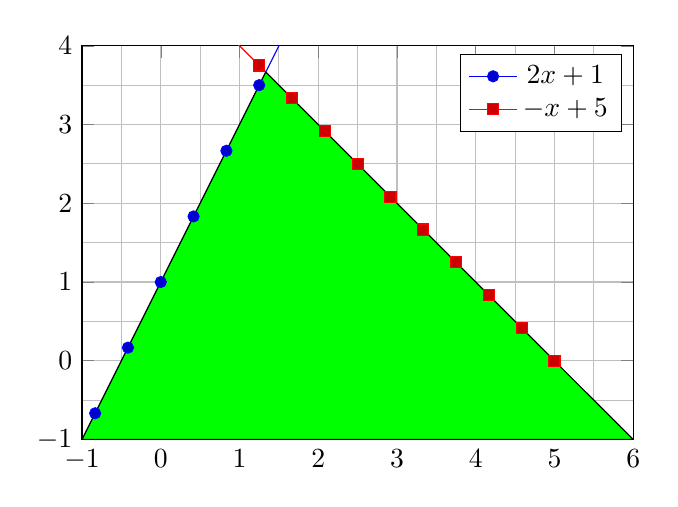
\begin{tikzpicture}
  \begin{axis}[
    xmin=-1,xmax=6,
    ymin=-1,ymax=4,
    x=1cm,
    y=1cm,
    minor tick num=1,% zwischen zwei Haupt-Achsmarkierungen jeweils einen Untermarkierungen einfügen
    minor tick length=0pt,% Länge der Untermarkierungen auf 0 setzen, sie also unterdrücken
    grid={both}% Gitterlinien sowohl durch die Positionen der Haupt- als auch Untermarkierungen
    ]
    \addplot{2*x+1};
    \addlegendentry{$2x+1$}
    \addplot{(-1)*x+5};
    \addlegendentry{$-x+5$}
    \addplot [fill=green] coordinates{(-1,-1) (1.333,3.666) (6,-1) (-1,-1)};
  \end{axis}
\end{tikzpicture}
\end{figure}
The whole green area lays "under" (because we have $<$) both functions which denotes that it contains all solution to satisfy both inequalities. We can see that for certain $y$-values only a handful $x$-values hold the inequalities. For example if $y$ has the value of $1$ then the inequalities only holds if $x\in ]0,4[$.\\
To adapt this idea onto our problem we consider for an assertion $x:succ(k\lesseqgtr l$) all assertions $x:succ(i\lesseqgtr j)$ such that by increasing $l$ the cardinality $i$ or $j$ also increases. Then we translate the cardinality constraints into a set of inequalities. For our two example above we have:\\
\begin{figure}[H]
\begin{minipage}[t]{.5\textwidth}
\raggedright
\begin{align*}
&2x\leq y\\
&3y\leq x\\
&1\leq x
\end{align*}
\end{minipage}%
\begin{minipage}[t]{.5\textwidth}
\raggedright
\begin{align*}
&x\leq 2y \\
&y\leq 3x \\
&1\leq x
\end{align*}
\end{minipage}
\end{figure}
By solving the system we get the following solution:
\begin{figure}[H]
\begin{minipage}[t]{.5\textwidth}
\raggedright
\centering
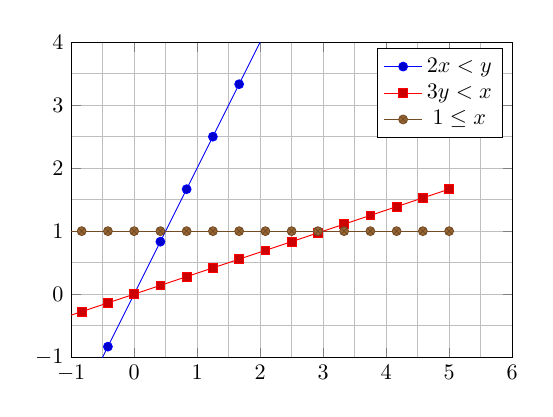
\begin{tikzpicture}[scale=0.8]
  \begin{axis}[
    xmin=-1,xmax=6,
    ymin=-1,ymax=4,
    x=1cm,
    y=1cm,
    minor tick num=1,
    minor tick length=0pt,
    grid={both}]
    \addplot{2*x};
    \addlegendentry{$2x<y$}
    \addplot{(1/3)*x};
    \addlegendentry{$3y<x$}
    \addplot{1};
    \addlegendentry{$1\leq x$}
  \end{axis}
\end{tikzpicture}
\end{minipage}%
\begin{minipage}[t]{.5\textwidth}
\raggedright
\centering
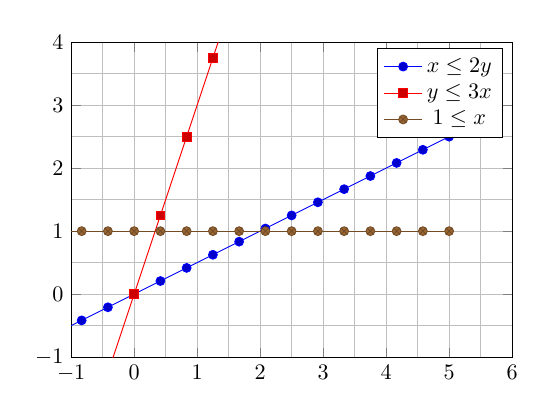
\begin{tikzpicture}[scale=0.8]
  \begin{axis}[
    xmin=-1,xmax=6,
    ymin=-1,ymax=4,
    x=1cm,
    y=1cm,
    minor tick num=1,
    minor tick length=0pt,
    grid={both}]
    \addplot{0.5*x};
    \addlegendentry{$x\leq 2y$}
    \addplot{3*x};
    \addlegendentry{$y\leq 3x$}
    \addplot{1};
    \addlegendentry{$1\leq x$}
  \end{axis}
\end{tikzpicture}
\end{minipage}
\end{figure}
If the solution is the empty set then there is no solution and our algorithm must block any attempts of satisfying any of this assertion by certain set terms. Those selected set terms are added to $b(S,x)$ before the algorithm starts. If the
solution is an interval then we have to look whether a natural number is existing in it.



 The increment depends on the non-blocked set term $u$ e.g. can not be formed from set terms in $b(S,x)$, for which we want to introduce a new variable $y$ and add $(x,y):u$ to $S$. To determine whether $u$ is \textit{safe} we count how often $u$ "appears" in $l$ and $k$. If it appears more often in $l$ than in $k$ then it is safe.
\begin{mydef}[Safe \RM{1}]
Let $x:succ(k\lesseqgtr l)$ be an assertion in $S$. Let $u=t_1\cap\dots \cap t_j$ with $1\leq i\leq j$. If $n_k(u)<n_l(u)$ and $u$ is not blocked by $x$ then $u$ is called \textit{safe regarding $k\leq l$}. The number $n_k(u)$ (and $n_l(u)$ respectively) is computed as followed:
\begin{algorithm}[H] \caption{Compute $n_k(u)$}
\begin{algorithmic}[l]
\State $n_k(u):=0$
\State $k=n_0+n_1\cdot|s_1|+\dots+n_j\cdot|s_j|$
\State $u=t_1\cap \dots \cap t_o$
\ForEach {$1\leq i\leq j:\, n_i\cdot|s_i|$, $s_i=s^\prime_1\cup \dots\cup s^\prime_p$, $p\in\mathbb{N}$}
\If {$\exists q, 1\leq q\leq p:$ $u=s^\prime_q\cap t^\prime$}
\State $n_k(u):=n_k(u)+n_i$
\EndIf
\EndFor\\
\Return $n_k(u)$
\end{algorithmic}
\end{algorithm}
\end{mydef}
This says that it is only safe to add a variable if $l$ increases faster then $k$.
As example we look at 
\begin{ex}
\begin{align*}
S=\{x:succ(|r\cup s|<|r|+|s|)\}
\end{align*}
\end{ex}
The set terms $r$ and $s$ are not blocked but still not safe because $n_{|r\cup s|}(r)=n_{|r|+|s|}(r)=1$ and $n_{|r\cup s|}(s)=n_{|r|+|s|}(s)=1$. However the set term $r\cap t$ is safe because $r\cap t\notin b(S,x)=\emptyset$ and $1=n_{|r\cup s|}(r\cap s)<n_{|r|+|s|}(r\cap s)=2$.\\
For an ABox where $k\leq l$ 
\subsection{Algorithm}
Finally we can present the Tableau-algorithm to determine the satisfiability of an ABox in $\mathcal{ALCSCC}$.
\begin{mydef}[Tableau]
Let $S$ be a set of assertions in simplified $NNF$.
\begin{enumerate}
\item\label{cap} $\sqcap$-rule: $S$ contains $x:C_1\sqcap C_2$ but not both $x:C_1$ and $x:C_2$\\
$\rightarrow$ $S:=S\cup\{x:C_1, x:C_2\}$
\item\label{cup} $\sqcup$-rule: $S$ contains $x:C_1\sqcup C_2$ but neither $x:C_1$ nor $x:C_2$\\
$\rightarrow$ $S:=S\cup\{x:C_1\}$ or $S:=S\cup\{x:C_2\}$
\item\label{choose}$choose$-rule: $S$ contains
\begin{itemize}
\item $x:succ(k\lesseqgtr l)$
\item $(x,y):k^\prime$, $k=n\cdot|k^\prime\cup u_1|+m\cdot|k^\prime\cap u_2|+u_3$, $n,m\in\mathbb{N}_0$, $u_1,u_2,u_3$ are set terms
\item but neither $(x,y):k$ nor $(x,y):k^\neg$
\end{itemize}
$\rightarrow$ either $S:=S\cup\{(x,y):k\}$ or $S:=S\cup\{(x,y):k^\neg\}$. Then jump to rule \ref{repeat}
\item\label{chooserole}$choose$-$a$-$role$-rule: $S$ contains $(x,y):s$ but for any $r\in\mathbf{R}$: $(x,y):r\notin S$\\
$\rightarrow$ choose $r\in\mathbf{R}$, such that $(x,y):r^\neg\notin S$. $S:=S\cup\{(x,y):r\}$. Then jump to rule \ref{repeat}
\item\label{dvd}$divide$-rule: $S$ contains $x:succ(n\,dvd\,l)$, $l=n_1\cdot|s_1|+\dots+n_i\cdot|s_i|+\dots+n_j\cdot|s_j|$, which is violated\\
$\rightarrow$ introduce a new variable $y$, choose $s=s_1\cap \dots \cap s_i$, $1\leq i\leq j$ and $S:=S\cup\{(x,y):s\}$. Then jump to rule \ref{repeat}
\item\label{leq}$\leq$-rule: $S$ contains 
\begin{itemize}
\item $x:succ(k\lesseqgtr l)$, which is violated
\item there is a set term $s:=|s_1\cap \dots \cap s_i|$, $l=n_1\cdot|s_1|+\dots+n_i\cdot|s_i|+\dots+n_j\cdot|s_j|$, which is safe regarding $k\lesseqgtr l$
\end{itemize}
$\rightarrow$ $S:=S\cup\{(x,y):s\}$. Then jump to rule \ref{repeat}
\item\label{exceeded}$merge$-rule: $S$ contains
\begin{itemize}
\item $x:succ(k\lesseqgtr l)$, which is violated
\item $(x,y_1):s_1$ and $(x,y_2):s_2$, such that $y_1\neq y_2$ and $k=n\cdot |s_1\cup s_2|+u$, where $u$ is a cardinality term
\end{itemize}
$\rightarrow$ merge $y_1$ and $y_2$ 
\item\label{s}$\leq 0$-rule: $S$ contains 
\begin{itemize}
\item $x:succ(|s_1\cap\dots\cap s_j|\leq 0)$
\item $(x,y):s_1$, $\dots$, $(x:y):s_i$, $1\leq i<j$
\item but not $(x,y):s_{i+1}$, $\dots$, $(x,y):s_j$
\end{itemize}
$\rightarrow$ choose $n\in\{i+1,\dots, j\}$, extend $S:=S\cup\{(x,y):s_n^\neg\}$ and then jump to rule \ref{repeat}
\item\label{repeat} $set.term$-rule (Repeat until inapplicable): In $S$ is $(x,y):s$ and
\begin{enumerate}
\item\label{setterm1} $s=s_1\cap s_2$ but $\{(x,y):s_1,\,(x,y):s_2\}\not\subseteq S$\\
$\rightarrow$ $S:=S\cup \{(x,y):s_1,\,(x,y):s_2\}$ 
\item\label{setterm2} $s=s_1\cup s_2$ and neither $\{(x,y):s_1\}\subseteq S$ nor $S\{(x,y):s_2\}\subset S$\\
$\rightarrow$ either $S:=S\cup \{(x,y):s_1\}$ or $S:=S\cup \{(x,y):s_2\}$ 
\item\label{setterm3} $s=C$ and $y:C\notin S$, where $C$ is an $\mathcal{ALCSCC}$ concepts\\
$\rightarrow$ $S:=S\cup\{y:C\}$
\end{enumerate}
\end{enumerate}
\end{mydef}
We now explain the rules of the Tableau-algorithm and their intention, if not already mention in Section \ref{restriction}.\\
The first rule decompose the conjunction and the second rule adds non-deterministically the right assertion.\\
The $choose$-rule is important because we need to know of every successor what kind of role successors and in which concepts they are. For an assertion $x:succ(k\lesseqgtr l$ it is important that $k^{\mathcal{I}(S)_x}$ and $l^{\mathcal{I}(S)_x}$ counts the successors correctly. In the following case the successor $y$ is not counted in $l^{\mathcal{I}(S)_x}:=(|r\cap s|^{\mathcal{I}(S)_x})$ while $x:succ(k\leq l)$ is violated.
\begin{ex}
\begin{align*}
S=\{x:succ(1\leq|r\cap s|), (x,y):r\}
\end{align*}
\end{ex}
There might be an model $\mathcal{I^\prime}$ where $y$ is also a $s$-successor of $x$ and hence $l^{\mathcal{I}(S)_x}<l^{\mathcal{I}^\prime(S)_x}$, which means that the assertion is in $\mathcal{I}^\prime$ satisfied, but in $\mathcal{I}(S)$ not. However the Tableau-algorithm should be able to construct every model of $S$ if $S$ is consistent. Therefore this rule adds non-deterministically either $(x,y):s$ or $(x,y):s^\neg$ which are the only two possibilities. This way we are also able to construct $\mathcal{I^\prime}$.\\
The $choose$-$a$-$role$-rule is necessary because in a ABox we may have assertions, which state that $x$ must have a successor but there are no assertions, which states what kind of successor it is. Hence we have to pick the \textit{right} role name. As example we have
\begin{ex}
\begin{align*}
&\mathbf{R}=\{r,s\}\\
&S=\{x:succ(|r^\neg|\leq 1)\}
\end{align*} 
\end{ex}
It states that $x$ have at least one successor which is not a $r$-successor. Since $\mathbf{R}$ only contains $r$ and $s$ we know that the successors must be an $s$-successor. First we apply rule \ref{leq} to actually add a successor. Therefore $y$ is introduced and $(x,y):r^\neg$ is added to $S$. Now no more rules are applicable except for the $choose$-$a$-$role$-rule. With that rule we can not pick $r$ because $r^\neg$ occurs in the assertion. Therefore we have to pick $s$. Another more simple but not so significant example is
\begin{ex}
\begin{align*}
&\mathbf{R}=\{r,s\}\\
&S=\{x:succ(|A|\geq 1)\}
\end{align*} 
\end{ex}
We know that $x$ must have a successor in $A$ but we still need to assign a role. In this case we can choose between $r$ and $s$.
\\
The $divide$-rule is straightforward: We choose one set term $s=s_1\cap\dots\cap s_i$ such that $l=n_1\cdot|s_1|+\dots+n_i\cdot|s_i|+\dots+n_j\cdot|s_j|$ and introduce a new variable $y$ and add $(x,y):s$ to $S$. For any $x:succ(n\,dvd\,l)$ we know that the chain of this rule application is finite because in worst case we have to introduce $n$ new variables with the same set term.
\\
The main idea of the $\leq$-rule is written in Section \ref{restriction}. We restrict the safeness criteria on the considered assertion $x:succ(k\lesseqgtr l)$ alone because sometimes it is unavoidable to increase the left hand side. This particular case is when we also have $x:succ(l\lesseqgtr k)$ in the same ABox. However we know that eventually we have $l^\prime=k^\prime$ because $l^\prime=l\cdot k$ and $k\prime\cdot l$.\\
The same goes for the $merge$-rule. We restrict the merging to the left hand side of cardinality constraints $k\lesseqgtr l$: It can be reasonable for the right hand side if by merging $l$ increases, for example $x:succ(1\leq |r\cap t|)$ with $(x,y_1):r$ and $(x,y_2):t$. However the easiest solution is just to add an $r\cap t$-successor. In case it is important to also restrict the number of $r\cap t$-successor e.g. $x:succ(|r\cap t|<2)$ we can define with the $choose$-rule whether $y_1$ and $y_2$ are also $r\cap t$-successor. And then with the assertion $x:succ(|r\cap t|<2)$ we can merge $y_1$ and $y_2$.\\
The $\leq 0$-rule deal with an assertion with a set constraint $s_1\subseteq s_2$, which is written here as cardinality constraint $|s_1\cap s_2^\neg|\leq 0$. Those cardinality constraint can not be dealt with the other rules. In case the left side has at least three set term  e.g. $|s_1\cap s_2\cap s_3|$ we have can have multiple possible solutions e.g. $(x,y):s_1\cap s_2\cap s_3^\neg$, $(x,y):s_1\cap s_2^\neg\cap s_3$ and $(x,y):s_1\cap s_2^\neg\cap s_3^\neg$. Hence we let the algorithm choose and backtrack if needed.\\
The $set.term$-rules are applied immediately after a new assertions $(x,y):s$ is added to $S$. The reason for that is, that we want to add all needed assertions for $y$ and hence update all $k^{\mathcal{I}(S)_x}$ correctly. We know that the number of this application is finite because an ABox is finite and hence the number of concept names and role names occurring in this ABox is also finite. Since the constraints are in $NNF$ set terms can never be infinite and hence this rule applies only a finite times.
\section{Correctness}
For the correctness proof of the Tableau-algorithm we have to show that
\begin{itemize}
\item For every input the Tableau-algorithm terminates
\item If no more rules are applicable on a clash-free ABox $S$ then $S$ is satisfiable
\item If $S$ is satisfiable then the Tableau-algorithm terminates without a clash
\end{itemize}
First we prove that the tableau algorithm terminates. 
\begin{mypro}
Let $C$ be a concept in simplified $CNNF$. Then there is no infinite chain of applications of any tableau rules issuing from $\{x:C\}$. 
\end{mypro}
\begin{mydef}[Derived Set]
A \textit{derived set} is an ABox $S^\prime$ where rule \ref{repeat} is not applicable.
\end{mydef}
In order words a derived set is an ABox on which we applied a rule completely e.g. every time we add a new assertion $(x,y):s$ we add all assertion concluded by it to $S$ (rule \ref{repeat}) first.\\
To prove this we map any derived set $S$ to an element $\Psi(S)$ from a set $Q$. We then show that the elements in $Q$ can be ordered by a well-founded relation $\prec$. A well-founded relation says that there is no infinite decreasing chain. If we can show that by obtaining a derived set $S^\prime$ from another set $S$ we have $\Psi(S^\prime)\prec\Psi(S)$ then the algorithm terminates.\\
The elements in $Q$ are finite multisets of septuples and the elements of the septuples are either integers or mutlisets of integers. For two septuples $q=(q_1,\dots,q_7)$ and $q^\prime=(q^\prime_1,\dots,q^\prime_7)$ it holds $q\prec q^\prime$ if for the first $i,\, 1\leq i\leq 7$, for which $q_i$ and $q_i^\prime$ differs it holds that $q_i\prec q_i^\prime$ (also called lexicographical ordering). For two mutlisets of integers $q_i$ and $q_i^\prime$ it holds $q_i^\prime\prec q_i$ if $q_i^\prime$ can be obtained from $q_i$ by replacing an integer $c$ in $q_i^\prime$ by a finite number of integers which are all smaller than $c$. The relation $\prec$ for those multisets is well-founded because we work with integers. That means from a multiset $\{0,\,\dots\,,0\}$ we can not obtain a smaller multiset because we would have to replace at least one $0$ with integers which are smaller.\\
For a concept $C$ its size $size(C)$ is inductively defined as
\begin{itemize}
\item $0$, if $C$ is $\perp$
\item $1$, if $C$ is a concept name of $\mathbf{C}$
\item $size(\neg C)= 1+size(C)$
\item $size(succ(c))= 1 + \sum_{C\in\mathbf{C}\text{ in c}} size(C)$
\item $size(C\sqcap D)=size(C\sqcup D)=size(C)+size(D)$
\end{itemize}
The asymmetrical difference of two numbers $n,m$ is denoted by 
\begin{equation*}
n\unlhd m \begin{cases}
n-m& \text{if } n> m\\
0 & \text{if } n\leq m
\end{cases}
\end{equation*}
The septuples in $Q$ are defined as follows
\begin{mydef}
Let $S$ be an ABox. The multiset $\Psi(S)$ consist of septuples $\psi_S(x)$ for each variable $x$. The component of the septuples are structured as follows
\begin{itemize}
\item the first component is a non-negative integer $max\{size(C)\mid x:C\in S\}$
\item the second component is a multiset of integers containing for each $x:C\sqcap D$, on which the $\sqcap$-rule is applicable, the non-negative integer $size(C\sqcap D)$ (respectively for $C\sqcup D$)
\item the third component is a multiset of integers containing for each $x:succ(k\lesseqgtr n)\in S$ the number of all successors $y$ of $x$ if rule \ref{choose} is applicable
\item the fourth component denotes the number of all successors of $x$.
\item the fifth component is a multiset which denotes for every $x:succ(k\lesseqgtr l)$ and $x:succ(n\,dvd\,l)$ the integer $k^{\mathcal{I}(S)_x}\unlhd l^{\mathcal{I}(S)_x}$ and $n\unlhd l^{\mathcal{I}(S)_x}$ respectively
\item the sixth component is the number of successors on which rule \ref{chooserole} is applicable
\item the seventh component is a multiset which denotes for each $x:succ(k\leq 0)$ the number of successors on which the rule \ref{leq} is applicable
\end{itemize}
\end{mydef}
\begin{mylem}
The following properties hold
\begin{enumerate}
\item For any concept $C$ we have $size(C)\geq size(NNF(\neg C))$
 \item Any variable $y$ in a derived set $S$ has at most one predecessor $x$ in $S$
\item If $(x,y):r\in S$ for a $r\in\mathbf{R}$ (and $y$ is a introduced variable) then 
\begin{align*}
max\{size(C)\mid x:C\in S\}>max\{size(D)\mid y:D \in S\}
\end{align*}
\end{enumerate}
\end{mylem}
\begin{proof}$ $\\
\vspace*{-5mm}
\begin{enumerate}
\item By induction over the number of applications to compute the negation normal form we have $size(C)=size(NNF(\neg C))$. Because $\neg succ(k\geq0)$ can be replace by $\perp$ which is $smaller$ than $\neg succ(k\geq 0)$, we have $size(C)\geq size(NNF(\neg C))$. This can be done because $\neg succ(k\geq 0)= succ(k<0)$ which is impossible to satisfy and therefore $\neg succ(k\geq 0)=\perp$.
\item If $y$ is a newly introduced variable, then it can only be introduced by exactly one variable $x$ which is $y$'s only predecessor. If two variables are merged together by rule \ref{exceeded} then both variables must have the same predecessor $x$ by the condition of that rule.
\item By the second fact we know that $x$ is the only predecessor of $y$. When $y$ is introduced by applying \ref{leq} on a assertion $x:succ(k\lesseqgtr l)$ then we have $y:C$ for every concept $C$ occurring in $l$ (for $\neg C$ we have $y:\neg C$). We know that $size(succ(k\lesseqgtr l))$ is greater then $size(C)=:max\{size(D)\mid y:D\in S\}$ therefore Lemma 1.3 holds. A new assertion $y:D$ can occur either because rule \ref{cap} or \ref{cup} are applicable on $y:C$ with $C=D\sqcap D^\prime$ or $C=D\sqcup D^\prime$, which neither raise $max\{size(D)\mid y:D \in S\}$, or because rule \ref{choose} is applicable but that also does not raise $max\{size(D)\mid y:D \in S\}$: If rule \ref{choose} is applicable on $x:succ(k\leq l)$ then for every added assertion $y:D$ the concept $D$ must occur in $k$ and therefore $size(succ(k\leq l))>size(D)$. If $y$ gets merged together with another variable $z$, then $y$ and $z$ must have the same predecessor which means that all concept sizes regarding $z$ are also smaller then $max\{size(C)\mid x:C\in S\}$. 
\end{enumerate}
\end{proof}
From the next Lemma we can conclude that the Tableau-algorithm terminates.
\begin{mylem}
If $S^\prime$ is a derived set obtained from the derived set $S$, then $\Psi(S^\prime)\prec\Psi(S)$
\end{mylem}
\begin{proof}
The following proof is sectioned by the definition of obtaining a derived set.
\begin{enumerate}
\item $S^\prime$ is obtained by the application of rule \ref{cap} on $x:C\sqcap D$:\\
The first component remains the same because $size(C)<size(C\sqcup D)$ and $size(D)<size(C\sqcap D)$. The second component decreases because rule \ref{cap} can not be applied on $x:C\sqcap D$ any more meaning that the corresponding entry in the multiset is removed. If $C$ (or $D$) happens to be a disjunction ($C^\prime\sqcup D^\prime$) or a conjunction ($C^\prime\sqcap D^\prime$) then the second component also becomes smaller because $size(C^\prime)$ and $size(D^\prime)$ are always smaller than the disjunction or conjunction of them and therefore also smaller than $size(C\sqcap D)$. Hence the entry for $size(C\sqcap D)$ can be replace by the smaller $size(C^\prime\sqcup D^\prime)$ or $size(C^\prime\sqcap D^\prime)$.\\
Consider now a tuple $\psi_S(y)$ such that $x\neq y$. $\psi_S(y)$ can only be affected if $x$ is a successor of $y$. The first and second component of $\psi_S(y)$ remain unaffected because both are independent from $x$. The third component of can never in creases because we do not add any new successors. If at all it can decreases because it may happen that by adding assertions regarding $x$ rule \ref{choose} can not be applied any more on some assertion $y:succ(k\lesseqgtr l)$. The fourth component does not change because we do not add any new successor. The fifth component can also only decrease but never increase: It can only increases if there is an assertion $y:succ(k\lesseqgtr l)$ and by adding $x:C$ or $x:D$ to $S$ we have $k^(\mathcal{I}(S^\prime)_y)-k^(\mathcal{I}(S)_y)>l^(\mathcal{I}(S^\prime)_y)-l^(\mathcal{I}(S)_y)$, which denotes that $k$'s increment was higher than $l$'s increment. However this 
This means that we can obtain $\Psi(S^\prime)$ from $\Psi(S)$ by replacing $\psi_S(x)$ with the smaller tuple $\psi_{S^\prime}(x)$. 
\item $S^\prime$ is obtained by the application of rule \ref{cup} on $x:C\sqcup D$:\\
similar to above
\item $S^\prime$ is obtained by the application of rule \ref{choose} on $x:succ(k\leq l)$ for a successor $y$ and of rule \ref{s}:\\
The first and second component of $\psi_S(x)$ do not change because this step only adds assertion regarding $y$. The third component becomes smaller because $y$ is not counted any more hence the number of successors for this assertion reduces in $\psi_S(x)$.\\
We consider now a tuple $\psi_S(z)$ such that $y\neq z$
\end{enumerate}
\end{proof}
\iffalse
\begin{mylem}
If the Tableau-algorithm terminates without a clash then $S$ is satisfiable
\end{mylem}
\begin{proof}$ $\\
Again the proof is sectioned by the obtained derived sets.\\
Let $\mathcal{I}(S^\prime)$ be the induced interpretation of the ABox $S^\prime$ created by the Tableau-algorithm from $S$. We show that $\pi_{\mathcal{I}(S^\prime)}$ satisfies $S^\prime$.\\
We start with the simple assertions $x:C$ and $(x,y):r$ for $C\in\mathbf{C}$ and $r\in\mathbf{R}$ (induction base): By the definition of induced interpretation we assign $\pi_{\mathcal{I}(S^\prime)}(x):=x^{\mathcal{I}(S^\prime)}\in C^{\mathcal{I}(S^\prime)}$. Also by the definition of induced interpretation for every $(x,y):r\in S^\prime$ we have $(\pi_{\mathcal{I}(S^\prime)}(x),\pi_{\mathcal{I}(S^\prime)}(y)):=(x^{\mathcal{I}(S^\prime)},y^{\mathcal{I}(S^\prime)})\in r^{\mathcal{I}(S^\prime)}$.\\
Let $S$ be an ABox and $\pi_{\mathcal{I}(S)}$ be an assignment which satisfies $S$ (induction hypothesis).\par
\begin{enumerate}
\item If we can apply rule \ref{cap} and obtain $S^\prime$ then there must be an assignment $x:C_1\sqcap C_2\in S$. By the definition of induced interpretation and by the hypothesis we already have $\pi_{\mathcal{I}(S^\prime)}(x)\in C_1^{\mathcal{I}(S^\prime)}$ and $\pi_{\mathcal{I}(S^\prime)}(x)\in C_2^{\mathcal{I}(S^\prime)}$. By adding $x:C_1$ and $x:C_2$ we do not change $\mathcal{I}(S)$. Hence $\mathcal{I}(S^\prime):=\mathcal{I}(S)$ and $\pi_{\mathcal{I}(S^\prime)}:=\pi_{\mathcal{I}(S)}$ satisfies $S^\prime$.
\item If we can apply rule \ref{cup} and obtain $S^\prime$ then there must be an assignment $x:C_1\sqcup C_2\in S$. Like above by the definition of the induced interpretation we have $\pi_{\mathcal{I}(S^\prime)}(x):=x^{\mathcal{I}(S^\prime)}$. We also know that $x^{\mathcal{I}(S^\prime)}$ is in $C_1^{\mathcal{I}(S^\prime)}\cup C_2^{\mathcal{I}(S^\prime)}$. By adding either $x:C_1$ or $x:C_2$ we do not change $\mathcal{I}(S)$. Hence $\mathcal{I}(S^\prime):=\mathcal{I}(S)$ and $\pi_{\mathcal{I}(S^\prime)}:=\pi_{\mathcal{I}(S)}$ satisfies $S^\prime$.
\item If we can apply rule \ref{choose} and obtain $S^\prime$ then we have an assertion $x:succ(k\leq l)$ and a successor $y$ such that $(x,y):k^\prime\in S$, $k^\prime$ occurs in $k$. We then choose between $(x,y):s$ and $(x,y):s^\neg$ for all $|s|$ in $k$ then apply rule \ref{repeat} until this rule is inapplicable. That means at the end we might add several assertions of the form $x:C$ and $(x,y):r$. In case we add $x:C$ we also add $x^{\mathcal{I}(S^\prime)}$ to $C^{\mathcal{I}(S^\prime)}$. Therefore in this case $\pi_{\mathcal{I}(S^\prime)}$ satisfies $S^\prime$. In case we add $(x,y):r$ we also add $(x^{\mathcal{I}(S^\prime)},y^{\mathcal{I}(S^\prime)})$ to $r^{\mathcal{I}(S^\prime)}$. Hence $\pi_{\mathcal{I}(S^\prime)}$ satisfies $S^\prime$.
\item If we can apply rule \ref{chooserole} and obtain $S^\prime$ then we have an assertion $(x,y):k$ but for every role name $r$ we do not have $(x,y):r\in S$, where $r$ has a positive sign in this assertion. After adding $(x,y):r$, $r\in\mathbf{R}$, to $S^\prime$ the element $(x^{\mathcal{I}(S)},y^{\mathcal{I}(S)})$ is also added to $r^{\mathcal{I}(S^\prime)}$. Hence $\pi_{\mathcal{I}(S^\prime)}$ satisfies $S^\prime$.
\item If we can apply rule \ref{leq} and obtain $S^\prime$ then we have an assertion $x:succ(c)$ such that it is violated regarding $x$.\\
We introduce $y$ and add $(x,y):l$ to $S$ and then apply rule \ref{repeat} until this rule is inapplicable. When we introduce $y$ we also add a new element $y^{\mathcal{I}(S^\prime)}$ to $\mathcal{I}(S^\prime)$. For each $y:C$ we add $y^{\mathcal{I}(S^\prime)}$ to $C^{\mathcal{I}(S^\prime)}$ and for each $(x,y):r$, $r\in\mathbf{R}$, we add $(x^{\mathcal{I}(S^\prime)},y^{\mathcal{I}(S^\prime)})$ to $r^{\mathcal{I}(S^\prime)}$. Therefore let $\pi_{\mathcal{I}(S^\prime)}:=\pi_{\mathcal{I}(S)}\cup \{y\mapsto y^{\mathcal{I}(S^\prime)}\}$.
\item If we can apply rule \ref{leq} and obtain $S^\prime$ then we have an assertion $x:succ(k<l)$ or $x:succ(k\leq l)$ such that it is violated regarding $x$. We also have two successors $y_1$ and $y_2$ for which $(x,y):s$ and $(x,y):s$ are in $S$.\\
If we merge both together to $y$ we also have to merge $y_1^{\mathcal{I}(S)}$ and $y_2^{\mathcal{I}(S)}$ to one element $y^{\mathcal{I}(S^\prime)}$. For each $y_i:C\in S$, $i\in\{1,2\}$ we have $y_i^{\mathcal{I}(S)}\in C^{\mathcal{I}(S)}$ and for each $(x,y_i):r$, $r\in\mathbf{R}$ we have $(x^{\mathcal{I}_S},y_i^{\mathcal{I}(S)})\in r^{\mathcal{I}(S)}$ due to the hypothesis. That means that by merging both elements the element $y^{\mathcal{I}(S^\prime)}$ must be in $C^{\mathcal{I}(S^\prime)}$ for every $y_i^{\mathcal{I}(S)}\in C^{\mathcal{I}(S)}$ and the element $(x^{\mathcal{I}(S^\prime)},y^{\mathcal{I}(S^\prime)})$ must be in $r^{\mathcal{I}(S^\prime)}$ for every $(x^{\mathcal{I}(S)},y_i^{\mathcal{I}(S)})\in r^{\mathcal{I}(S)}$. Therefore let $\pi_{\mathcal{I}(S^\prime)}:=\pi_{\mathcal{I}(S)}\backslash\{y_1\mapsto y_1^{\mathcal{I}(S)}, y_2\mapsto y_2^{\mathcal{I}(S)}\}\cup\{y\mapsto y^{\mathcal{I}(S)}\}$ which satisfies $S^\prime$.
\item If we can apply rule \ref{s} and obtain $S^\prime$ then we have an assertion $x:succ(c_1\subseteq c_2)$ and a successor $y$ such that $(x,y):c_1\in S$ but $(x,y):c_2\notin S$. By adding $(x,y):c_2$ to $S$ we have also to add $y:C$ for every concept $C$ in $c_2$ and $(x,y):r$ for every role name $r$ in $c_2$. That means that $x^{\mathcal{I}(S)}$ is added to every $C^{\mathcal{I}(S)}$ and that $(x^{\mathcal{I}(S)},x^{\mathcal{I}(S)})$ is added to every $r^{\mathcal{I}(S)}$. Therefore the assignment $\pi_{\mathcal{I}(S^\prime)}:=\pi_{\mathcal{I}(S)}$ satisfies $S^\prime$.
\end{enumerate}
\end{proof}
\begin{mylem}
If $S$ is satisfiable then the Tableau-algorithm terminates without a clash.
\end{mylem}
\begin{proof}
\end{proof}
\fi
\normalem
\bibliographystyle{abbrv}
\bibliography{ref}
\end{document}
